\newbox\FishingTool
\sbox\FishingTool{%
\begin{tikzpicture}
	\clip 	[rounded corners=.5cm] (0,0) rectangle (2,2);
	\node 	[minimum size=2cm, inner sep=0pt,outer sep=0pt,clip] (image) at (1,1) {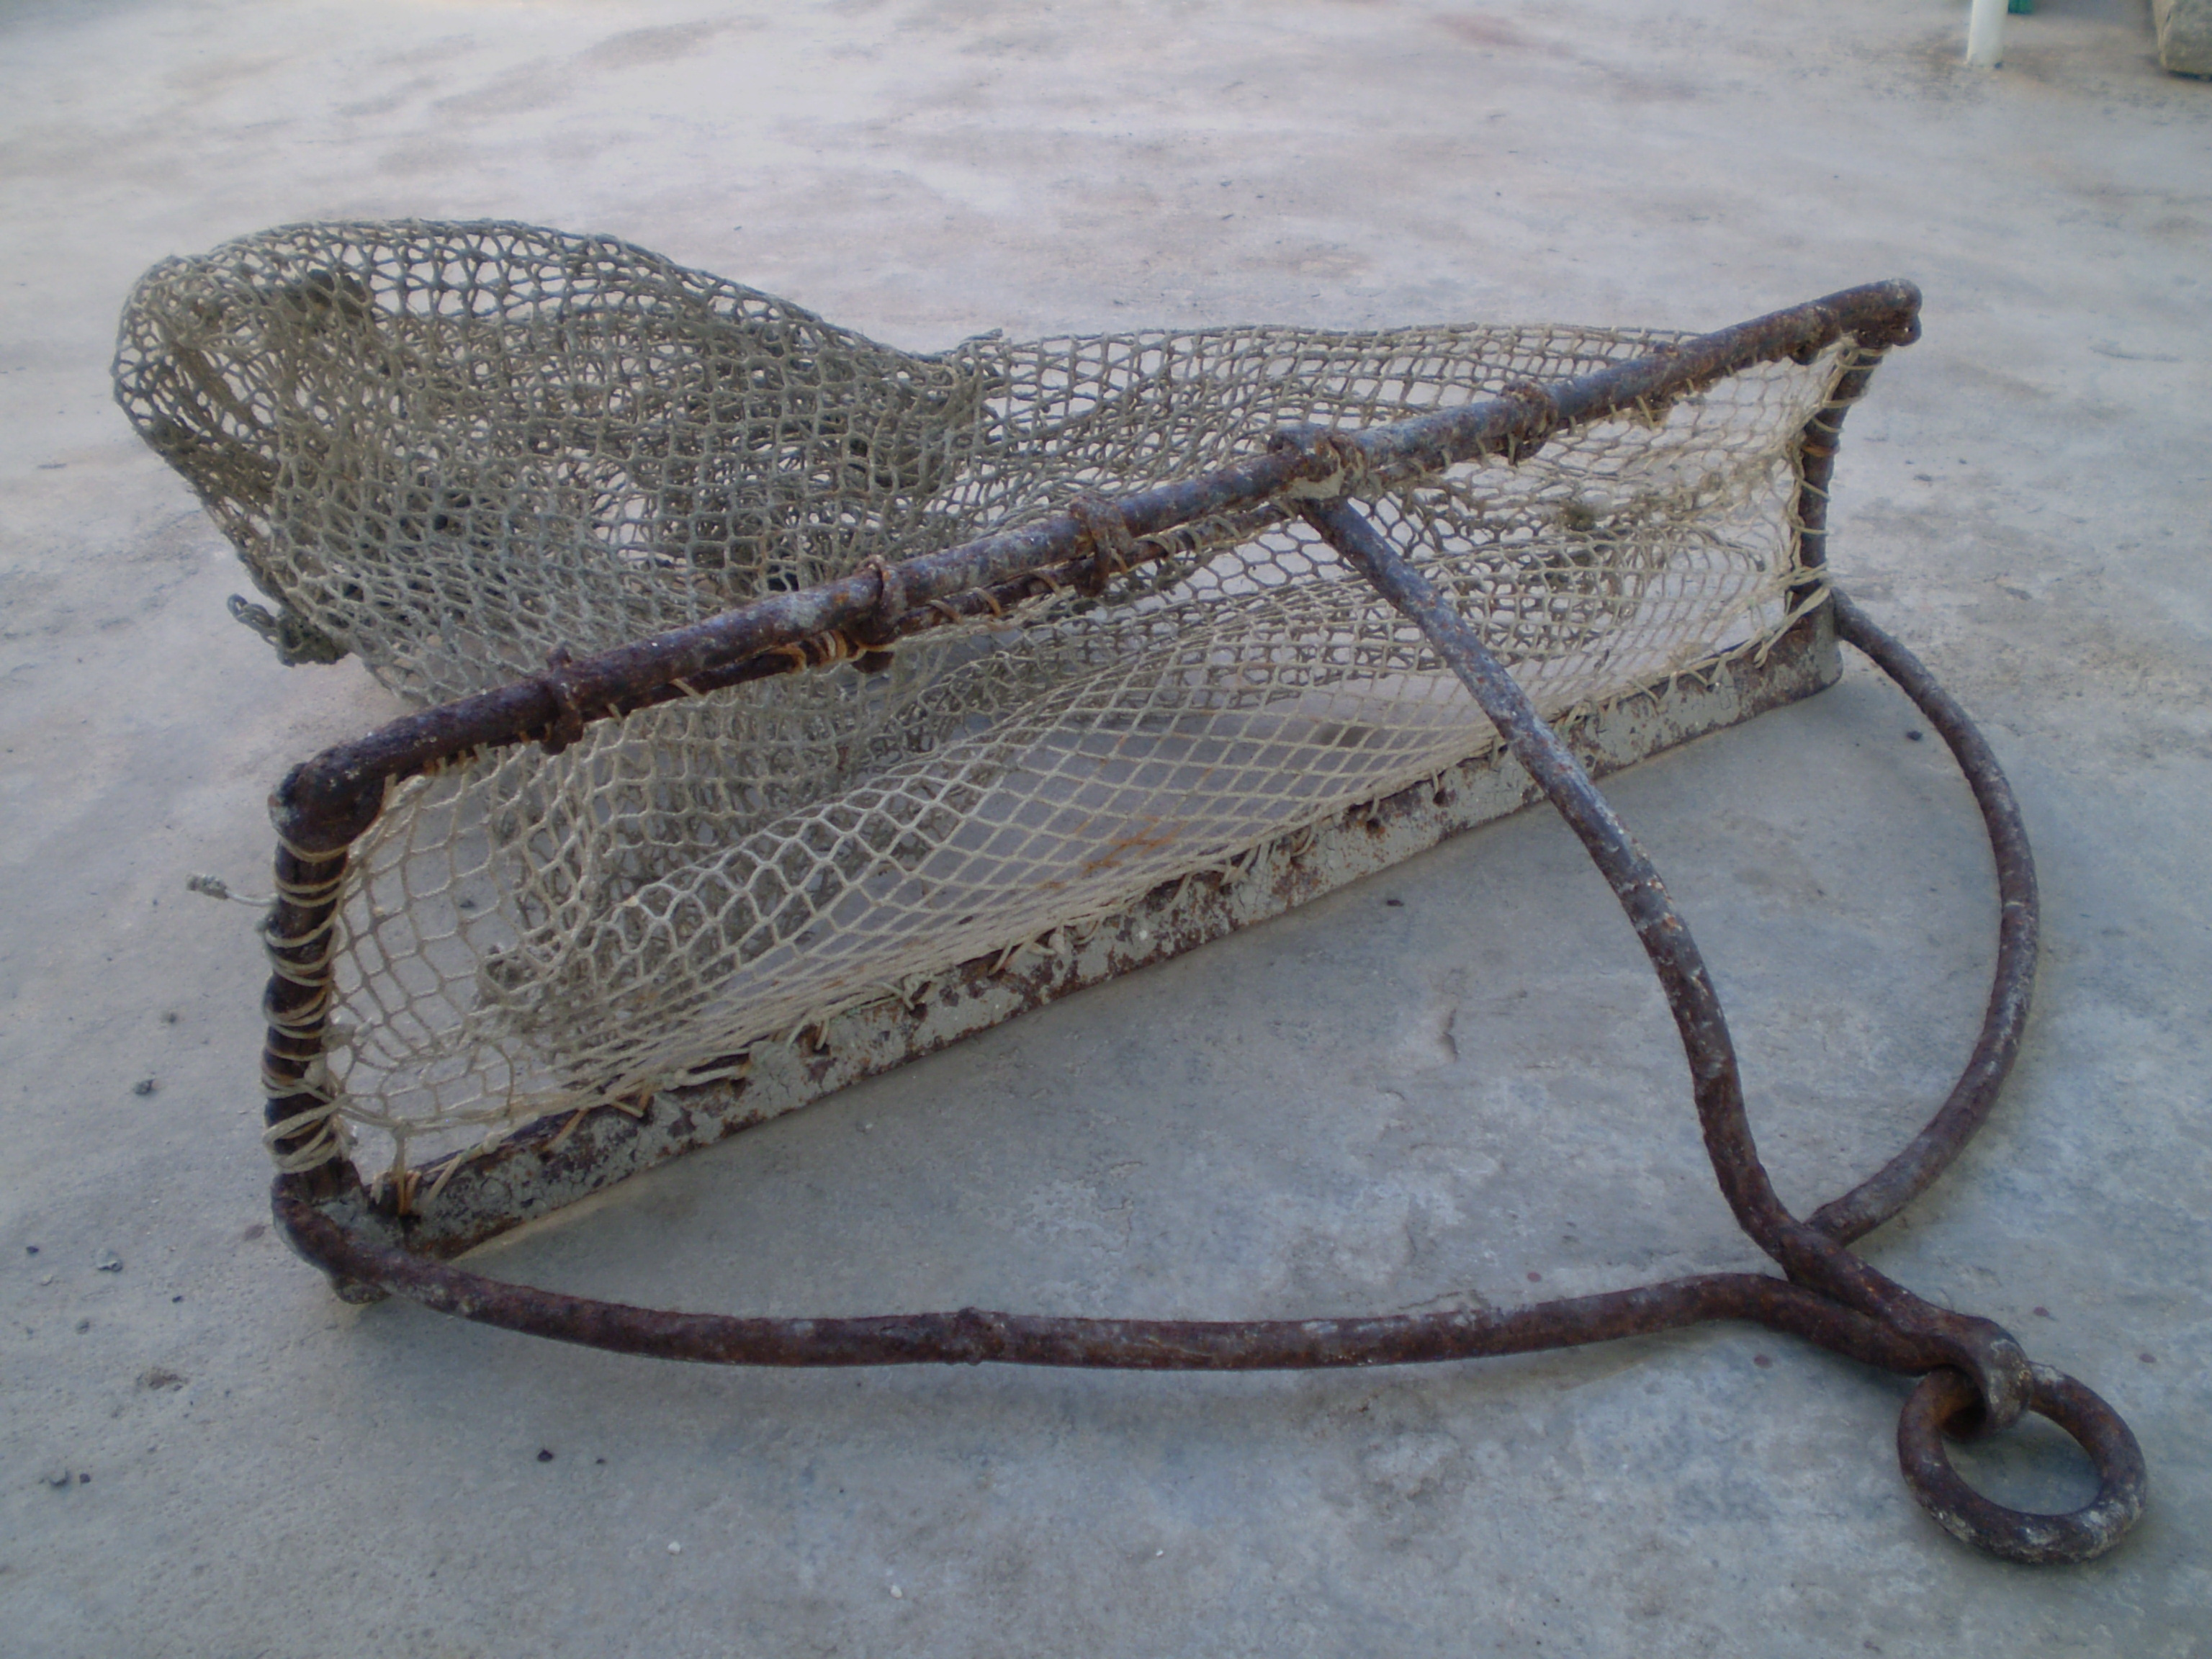
\includegraphics[height=2cm]{illustrations/skevin_fig4_brganja.jpg}};
	\draw 	[rounded corners=.5cm]
			([shift={(0.5\pgflinewidth,0.5\pgflinewidth)}]0,0) rectangle
			([shift={(-0.5\pgflinewidth,-0.5\pgflinewidth)}]2,2);
\end{tikzpicture}}

\newbox\OtherFishingTool
\sbox\OtherFishingTool{%
\begin{tikzpicture}
	\clip 	[rounded corners=.5cm] (0,0) rectangle (2,2);
	\node 	[minimum size=2cm, inner sep=0pt,outer sep=0pt,clip] (image) at (1,1) {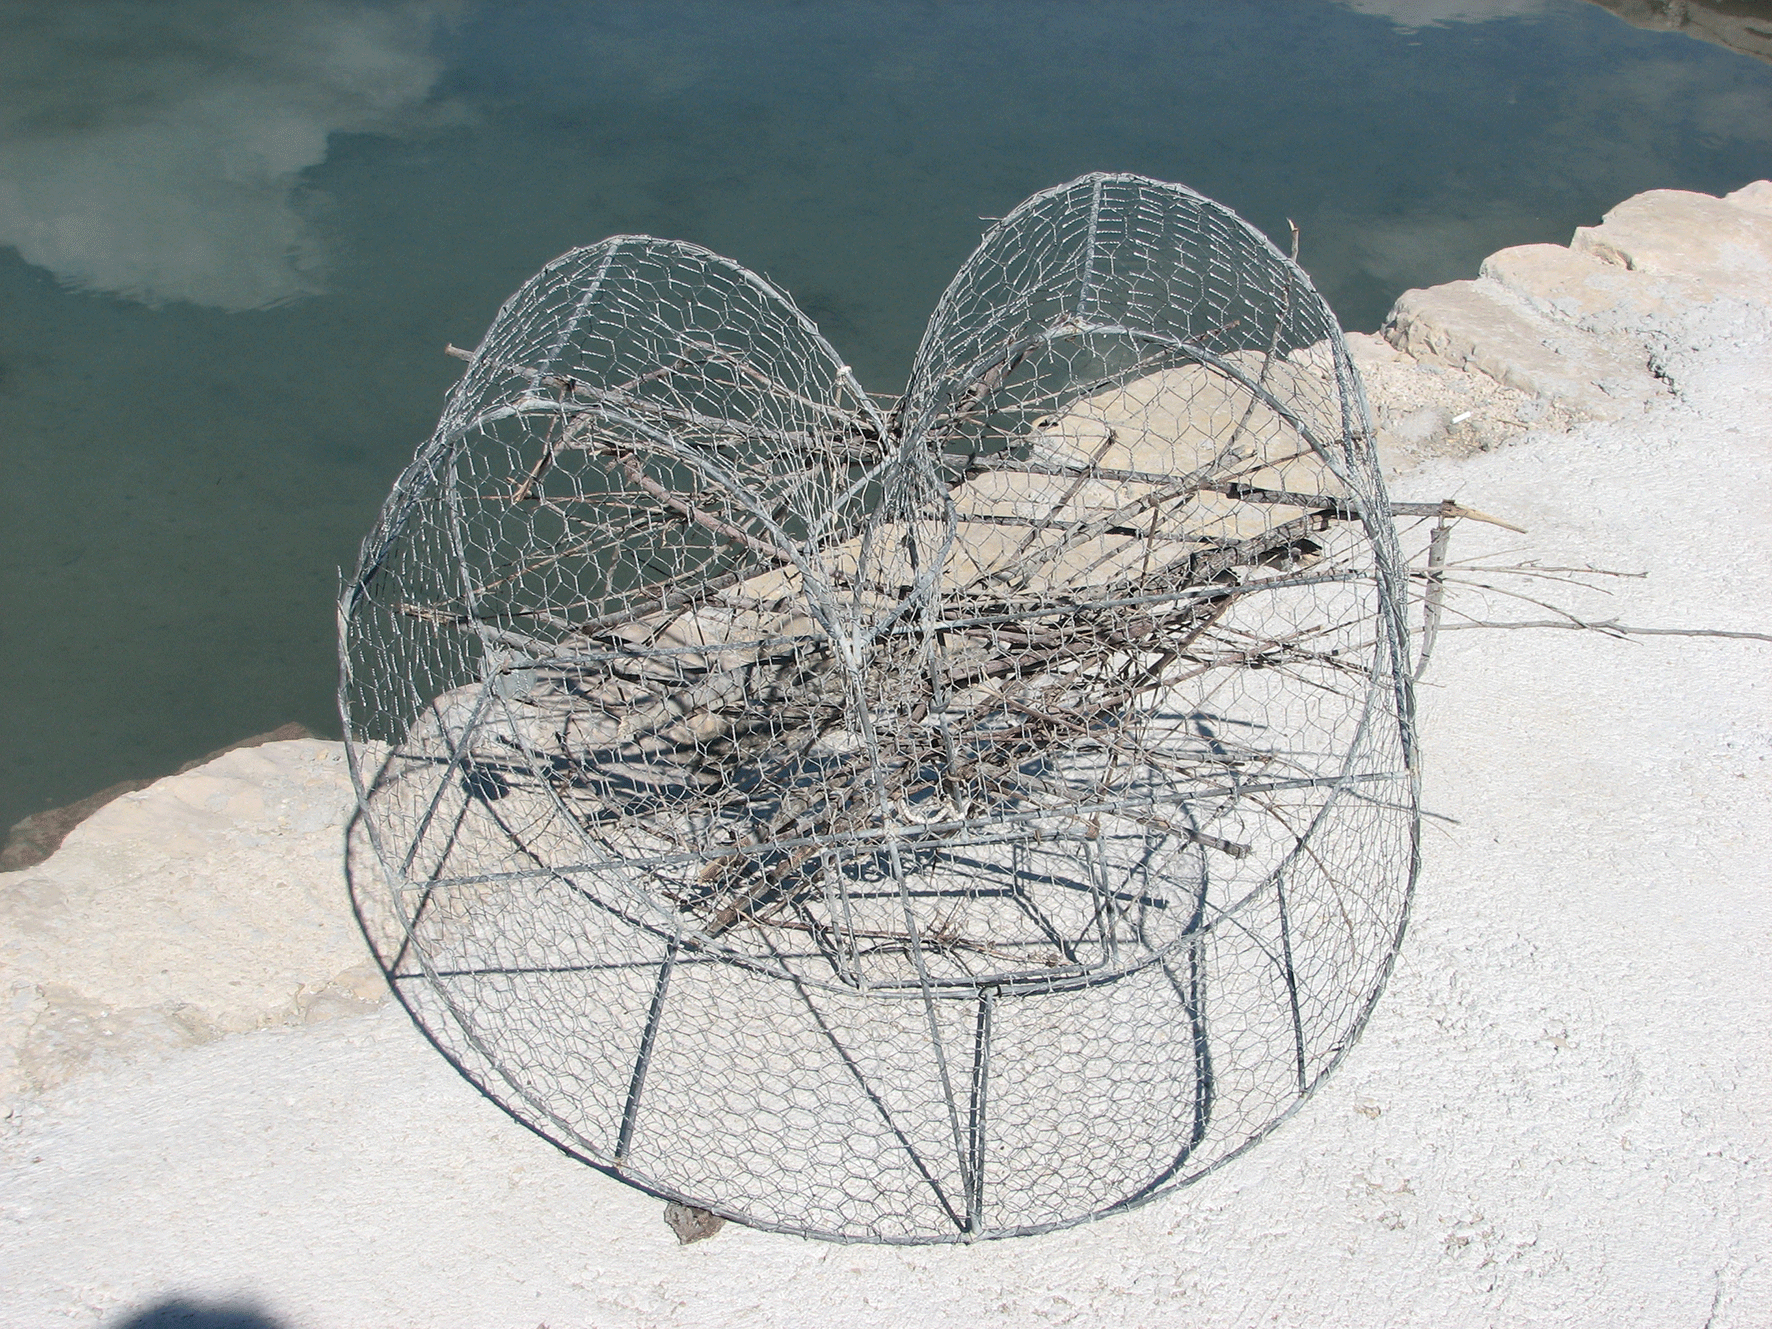
\includegraphics[height=2cm]{illustrations/skevin_fig4_vrsa}};
	\draw 	[rounded corners=.5cm]
			([shift={(0.5\pgflinewidth,0.5\pgflinewidth)}]0,0) rectangle
			([shift={(-0.5\pgflinewidth,-0.5\pgflinewidth)}]2,2);
\end{tikzpicture}}


\newcommand*{\BrganjaOldSpeakers}[1]{%
\begin{tikzpicture}
	[
		scale=#1,
		every node/.style={
			anchor=base,
			minimum height=\ht\FishingTool,
			text centered,
			fill=white,
			transform shape
		}
	]
	\node	[align=center,draw,rounded corners=.25cm] (trans) at (3,3) {`A type of a fishing tool\\used to collect different kinds\\of seashells by dragging it\\across the sea floor.'};
	\node	[below left = 2.5cm of trans,draw] (native) at (2,0) {\itshape\textbf{brganja} f.};
	\node	[below right = 2.5cm of trans,inner sep=0pt,outer sep=0pt] (image) at (4,0) {\usebox\FishingTool};
	\begin{scope}[on background layer]
		\draw	(native.west) to (trans.north);
		\draw	(image.east) to (trans.north);
		\draw	(native.west) to (image.east);
	\end{scope}
\end{tikzpicture}}

\newcommand*{\BrganjaYoungAdults}[1]{%
\begin{tikzpicture}
	[
		scale=#1,
		every node/.style={
			anchor=base,
			minimum height=\ht\OtherFishingTool,
			text centered,
			fill=white,
			transform shape
		}
	]
	\node	[align=center,draw,rounded corners=.25cm] (trans) at (3,3) {`A net used for\\collecting seashells.'};
	\node	[below left = 2.5cm of trans,draw] (native) at (2,0) {\itshape\textbf{brganja} f.};
	\node	[below right = 2.5cm of trans,inner sep=0pt,outer sep=0pt] (image) at (4,0) {\usebox\OtherFishingTool};
	\node 	[right = 0em of image,draw,yshift=-10pt] (unsure) {\bfseries ?};
	\node	[left = 0em of image,inner sep=0pt,outer sep=0pt,yshift=-10pt] (FishingTool) {\usebox\FishingTool};
	\begin{scope}[on background layer]
		\draw	(native.west) to (trans.north);
		\draw	(image.east) to (trans.north);
		\draw	(native.west) to (image.east);
	\end{scope}
\end{tikzpicture}}

\newcommand*{\BrganjaYoungAdultsSemanticExtension}[1]{%
\begin{tikzpicture}
	[
		scale=#1,
		every node/.style={
			anchor=base,
			minimum height=\ht\OtherFishingTool,
			text centered,
			fill=white,
			transform shape
		}
	]
	\node	[align=center,draw,rounded corners=.25cm] (trans) at (3,3) {`A net used for\\collecting seashells.'};
	\node	[right = 1.5cm of trans,align=center,draw,rounded corners=.25cm] (SemanticExtension) {`A summer festivity\\celebrated every first\\Sunday in August.'};
	\node	[below left = 2.5cm of trans,draw] (native) at (2,0) {\itshape\textbf{brganja} f.};
	\node	[below right = 2.5cm of trans,inner sep=0pt,outer sep=0pt] (image) at (4,0) {\usebox\OtherFishingTool};
	\node 	[right = 0em of image,draw,yshift=-10pt] (unsure) {\bfseries ?};
	\node	[left = 0em of image,inner sep=0pt,outer sep=0pt,yshift=-10pt] (FishingTool) {\usebox\FishingTool};
	\draw[vecArrowOlive] (trans) to (SemanticExtension);
	\draw[vecOpenArrowRed] (trans) to (SemanticExtension);
	\draw[innerOlive] (trans) to (SemanticExtension);
	\begin{scope}[on background layer]
		\draw	(native.west) to (trans.north);
		\draw	(image.east) to (trans.north);
		\draw	(native.west) to (image.east);
	\end{scope}
\end{tikzpicture}}


	% To get "Young adults: semantic extension" to span 
	% the last two subfigures, I've put stuff inside of
	% minipages on top of the subfigures. This is a bit of
	% hack, in my opinion, because it separates content
	% that forms a logical group, but I can't really think
	% of a better alternative. 
	\begin{minipage}[t]{0.29\textwidth}
		\centering
		\textbf{Older speakers}
	\end{minipage}%
	\hspace{.05\textwidth}%
	\begin{minipage}[t]{0.63\textwidth}
		\centering
		\textbf{Young adults: semantic extension}
	\end{minipage}%
	\newline\newline%
	%
	\begin{subfigure}[t]{0.29\textwidth}
		{\centering
		\BrganjaOldSpeakers{0.3}}
		
		 This is a triadic relation formed in the mind of an older speaker but not in the minds of the young informants.
		 This word has a different effect on young speakers.
	\end{subfigure}%
	\hspace{.05\textwidth}%
	\begin{subfigure}[t]{0.29\textwidth}
		{\centering
		\BrganjaYoungAdults{0.3}}
		
		This is a triadic relation formed in the mind of a young speaker.
		The second element of Peirce's semiotic triangle, the \emph{thing signified} or \emph{referential object}, varies.
		Five out of seven speakers are unsure about the correct referential object; they either describe another fishing tool, or they don't know how to describe it.
		But all of them, without exception, know its function.
		Thus, communication is still fulfilled at the pragmatic level.
	\end{subfigure}%
	\hspace{.05\textwidth}%
	\begin{subfigure}[t]{0.29\textwidth}
		{\centering
		\BrganjaYoungAdultsSemanticExtension{0.3}}
		
		Young speakers know this word thanks to the fact that the community of Betina has refunctionalized it; that is, it has changed its function and accordingly its semiotic space.
		This word traditionally signified a tool which for centuries was used by the inhabitants of Betina on a daily basis, mostly to get food.
		A few decades ago, a new substance was attributed to this word: the value of tradition and of collective memory through the name of the festival \emph{Dan Brganje} (Brganja Day).
	\end{subfigure}%

